%----------------------------------------------------------------------------------------
%	SECTION 1
%----------------------------------------------------------------------------------------

\section{The Independence and Circuit Axioms.}

\begin{definition}
    A \textbf{matroid} $M$, on a finite set $E$, called the \textbf{ground set}
    is  a pair $(E,\Ic)$ where $\Ic \subseteq 2^E$ is a collection of
    \textbf{independent sets}, such that:
    \begin{enumerate}
        \item[(I1)] $\emptyset \in \Ic$.

        \item [(I2)] If $I_1 \in \Ic$, and  $I_2 \subseteq I_1$, then  $I_2 \in
            \Ic$.

        \item[(I3)] If $I_1,I_2 \in \Ic$, and  $|I_1|<|I_2|$, then there exists
            an  $e \in \com{{I_2}}{I_1}$ such that $I_1 \cup e \in \Ic$.
    \end{enumerate}
    We call properties (I2) and (I3) the \textbf{inheretence} and
    \textbf{augmentation} axioms, respectively.
\end{definition}

\begin{example}\label{1.1}
    \begin{enumerate}
        The emptyset $\emptyset$ together with $2^\emptyset=\{\emptyset\}$ forms
        a matroid called the \textbf{empty matroid} and the collection $2^E$ on an
        nonempty set $E$ induces a matroid called the \textbf{trivial matroid}.
        It is easy to see why these two are matroids; since one encompasses only
        the empty set, and the other all subsets, these two matroids are not
        very interesting.
    \end{enumerate}
\end{example}

We provide some equivalent definitions with independent sets.

\begin{example}\label{1.2}
    \begin{enumerate}
        \item[(1)] Let $E$ be a finite set. Then $M=(E,\Ic)$ is a matroid if,
            and only if:
            \begin{enumerate}
                \item[(I^{\prime}1)] $\Ic \neq \emptyset$.

                \item[(I^{\prime}2)] Inheritance holds.

                \item[(I^{\prime}3)] If $I_1,I_2 \in \Ic$, with $|I_2|=|I_1|+1$,
                    then there is an $e \in \com{I_2}{I_1}$ such that $I_1 \cup e
                    \in \Ic$.
            \end{enumerate}

        Notice, that if $M$ is a matroid, then  $\emptyset \in \Ic$, so  (1) is
        satisfied. Moreover, the augmentation theorem implies (3), since if
        $|I_2|=|I_1|+1$, we have $|I_1|<|I_2|$.

        On the otherhand, if $\Ic \neq \emptyset$, then $\Ic$ contains, at least
        $\emtyset$, since  $\Ic \subseteq 2^E$. (I2) is also given by (2).

        Now, if $I_1, I_2 \in \Ic$ such that $|I_2|=|I_1|+1$, then $|I_1|<|I_2|$,
        and it follows from there that (3) implies (I3).

        This gives us an equivalent way to define the matroid $M$, still using
        independent sets, but with different rules.

    \item[(2)] A finite set $E$ together with a collection  $\Ic \subseteq 2^E$
        is a matroid if, and only if the following hold:
        \begin{enumerate}
            \item[(I^{\prime\prime}1)] $\emptyset \in \Ic$.

            \item[(I^{\prime\prime}2)] Inheritance holds; i.e. if $I \in \Ic$
                and  $J \subseteq I$, then  $J \in \Ic$.

            \item[(I^{\prime\prime}3)] If $X \subseteq E$, and  $I_1,I_2 \in
                \Ic$ are maximal such that $I_1,I_2 \subseteq X$ (that is, $I_1$
                and $I_2$ are maximal sets of the collection $\{I \in \Ic :
                I \subseteq X\}$), then $|I_1|=|I_2|$.
        \end{enumerate}

        It is rather simple to prove (1) and (2), so the nontrivial work
        goes to showing that property (3) and (I3) are equivalent to each
        other.
    \end{enumerate}
\end{example}

\begin{definition}
    Let $M=(E,\Ic)$ be a matroid. A subset of $E$ that is not independent, i.e.
    $X \subseteq E$ with  $X \notin \Ic$ is called a \textbf{dependent set}.
\end{definition}

the following example shows why Whitney gave the name ``matroid'' to these
structures.

\begin{example}\label{1.4}
    \begin{enumerate}
        \item[(1)] Consider an $m \times n$ matrix  $A \in F^{m \times n}$,
            where $F$ is a field. Define $E$ to  be the set of all column labels
            of the matrix $A$, i.e.  $A=\{1, \dots, m\}$ and define $\Ic
            \subseteq 2^E$ to be the collection of all multisets of $E$
            linearly independent over $F^{m \times n}$ considered as a vector
            space. Then $M=(E,\Ic)$ is a matroid.

            First notice that $\emptyset$ is trivially linearly independent, so
             $\emptyset \in \Ic$. Moreover, if $I_1 \in \Ic$ is linearly
             independent, and $I_2 \subseteq I_1$, then $I_2$ is also linearly
             independent, so  $I_2 \in \Ic$.

             Now, let $X,Y \in \Ic$ be linearly independent with $|X|<|Y|$, and
             consider the subspace $W \subseteq F^{m \times n}$ spanned by $X
             \cup Y$; i.e. $\Span{W}=X \cup Y$. then $\dim{W} \geq |Y|$. Now,
             suppose tht $X \cup i$ is linearly dependent for all  $i \in
             \com{Y}{X}$, then $W \subseteq \Span{X}$, thus $\dim{W} \leq
             |X|<Y$, which is a contradiction. Thus, there is atleast one $i \in
             \com{Y}{X}$ for which $X \cup i \in \Ic$. This makes $M$ a matroid
             which we call the  \textbf{vector matroid} over $A$, and we denote
             it $M[A]$.

         \item[(2)] Let
             \begin{equation*}
                 A=\begin{pmatrix}
                    1   &   0   &   0   &   1   &   1   \\
                    0   &   1   &   0   &   0   &   1   \\
                   \end{pmatrix}
             \end{equation*}
             be a $2 \times 5$ matrix on $\R$. Then considering the vector
             matroid over $M$ oveer  $A$, with $E=\{1,2,3,4,5\}$, we get the
             independent sets are:
             \begin{align*}
                 \{1\}  && \{2\} && \{4\} && \{1,2\} \\
                \{1,5\} && \{2,4\} && \{2,5\} && \{4,5\} \\
             \end{align*}
             The collection of dependent sets are:
             \begin{align*}
                 \{3\} && \{1,3\} && \{1,4\} && \{2,3\} \\
                 \{3,4\} && \{3,5\} && \{1,2,5\} && \{2,4,5\} \\
             \end{align*}
    \end{enumerate}
    The minimal dependent sets of $M$ on  $A$ is:
    \begin{align*}
        \{3\} && \{1,4\} && \{1,2,5\} && \{2,4,5\} \\
    \end{align*}
\end{example}

\begin{remark}
    Since matroids are a pair of a ground set $E$ and a subset of $2^E$ we can
    usually just specify the matroid by $E$ and take the collection of
    independent sets (or another collection) to be imposed.
\end{remark}

\begin{lemma}\label{1.1.1}
    Let $E$ be a subset of a vector space  $V$, and let  $\Ic$ be the collection
    of all linearly independent subsets of  $E$. Then  $E$, together with  $\Ic$
    forms a matroid.
\end{lemma}
\begin{proof}
    The proof of example \ref{1.3}(1) can be repeated. In fact, notice that an $m
    \times n$ matrix is just a collection of  $n$ vectors of length  $m$ in
    $F^m$. We now prove this for arbitrary vector spaces.

    $\emptyset$ is trivially linearly independent, so  $\emptyset \in \Ic$;
    moreover, if  $I_1$ is a set of linearly independnet vectors, and $I_2
    \subseteq I_1$, then $I_2$ is also linearly independent; so inheritance
    holds.

    Now, let $I_1=\{v_1, \dots, v_m\}$, and $I_2=\{u_1, \dots, u_n\}$ be
    linearly independent sets of vectors with $n<m$. Then  $|I_2|<|I_1|$, with
    $u_i=v_i$ possibly equal for some  $1 \leq i \leq n$. Then, there exists some
    $v_j \in \com{I_1}{I_2}$ distinct from all other $u_i$. Now, suppose that
    $I_2 \cup v_j$ is linearly dependent. Then  we have
    \begin{equation*}
        \alpha_1u_1+\dots+\alpha_nu_n+\alpha v_j = 0
    \end{equation*}
    which implies that $\alpha \neq 0$. So we get:
    \begin{equation*}
        v_j=\inv{\alpha}\alpha_1u_1+\dots+\inv{\alpha}\alpha_nu_n
    \end{equation*}
    This puts $v_j \in \Span{I_2}$, thus $\com{I_1}{I_2} \subseteq \Span{I_2}$,
    thus $(\com{I_1}{I_2}) \cup I_2=I_1 \subseteq \Span{I_2}$. This makes
    $|I_1|<|I_2|$; but $|I_2|<|I_1|$, a contradiction. Therefore $I_2 \cup v_j$
    must be linearly independent. This makes $E$ into a matroid.
\end{proof}
\begin{remark}
    Most notably, if $V$ is a vector space, then  $V$ together with the
    collection of all linearly independent subsets forms a matroid.
\end{remark}

\begin{definition}
    We call a matroid $M$ \textbf{vectorial} if its ground set is a subset of a
    vector space $V$ and the collection of independent sets consist of all
    linearly independent subsets of $V$.
\end{definition}

\begin{definition}
    We call a minimal dependent set of a matroid $M$ a  \textbf{circuit}. If $C$
    is a circuit of size  $|C|=n$, we call  $C$ an  $n$-circuit. We denote the
    collection of all circuits of  $M$ by  $\Cc$.
\end{definition}

This definition will also provide us with an alternative definition for a
matroid.

\begin{lemma}[The Circuit Axioms.]\label{1.1.2}
    The collection $\Cc$ of circuits of a matroid satisfy the following:
    \begin{enumerate}
        \item[(C1)] $\emptyset \notin \Cc$.

        \item[(C2)] If $C_1, C_2 \in \Cc$, and $C_1 \subseteq C_2$, then
            $C_1=C_2$.

        \item[(C3)] If $C_1, C_2 \in \Cc$ are distinct, and $z \in C_1 \cap
            C_2$, then there exists a circuit $C \in \Cc$ such that $C \subseteq
            \com{(C_1 \cup C_2)}{z}$.
    \end{enumerate}
\end{lemma}
\begin{proof}
    If $M$ is a matroid with  $\Ic$ the collection of independent sets, then
    $\emptyset \in \Ic$, by definition, this makes  $\emptyset \notin \Cc$.
    Moreover, if $C_1,C_2 \in \Cc$ are circuits, then they are minimally
    dependent, so if $C_1 \subseteq C_2$, it must be that $C_1=C_2$, otherwise
    we would have $C_1 \in \Ic$, a contradiction.

    Now, let $C_1,C_2 \in \Cc$ be distinct circuits, and let $z \in C_1 \cap
    C_2$. Now, suppose that $\com{(C_1 \cup C_2)}{z}$ does not contain a
    circuit; then $\com{(C_1 \cup C_2)}{z} \in \Ic$, Now, by the above, (C2),
    we have $\com{C_2}{C_1} \neq \emptyset$, so choose an $f \in \com{C_2}{C_1}$.
    By minimality, we have $\com{C_2}{f} \in \Ic$, so choose a maximally
    independent subset $I \suseteq C_1 \cup C_2$ such that $\com{C_2}{f}
    \subseteq I$. Then $f \notin I$; and since  $C_1$ is a circuit, for some $g
    \in C_1$, $g \notin I$, moreover,  $g \neq f$. Therefore, we have:
    \begin{equation*}
        |I| \leq |\com{(C_1 \cup C_2)}{\{f,g\}}|=|C_1 \cup C_2|-2 \leq
        |\com{(C_1 \cup C_2)}{z}|=|C_1 \cup C_2|-1
    \end{equation*}
    By the augmentation axiom (I3), let $I_1=I$, $I_2=\com{(C_1 \cup C_2)}{z}$,
    then we get $I_1 \cup g \in \Ic$ which contradicts the maximality of $I$.
\end{proof}
\begin{remark}
    This just establishes the validity of the circuit axioms for matroids. To
    actually show that these axioms provide an equivalent definition, we need
    the following theorem, and its corollary.
\end{remark}

\begin{theorem}\label{1.1.3}
    Let $E$ be a finite set having  $\Cc \subseteq 2^E$ satisfying (C1)-(C3).
    Let $\Ic$ be the collection of all subsets of $E$ which don't contain
    elements of  $\Cc$; i.e.
    \begin{equation*}
        \Ic=\{X \subseteq E : Y \notin \Cc \text{ given } Y \subseteq X\}
    \end{equation*}
    Then $\Ic$ defines the collection of independent sets of a matroid on $E$.
\end{theorem}
\begin{proof}
    Notice that $\emptyset$ contains no subsets of  $E$ contained in  $\Cc$, so
     $\emptyset \in \Ic$; furthermore, if  $I_1 \in \Ic$ contains no subsets of
     $E$ contained in  $\Cc$, neither does a subset  $I_2 \subseteq I_1$, so
     $I_2 \in \Ic$.

     Now, let $I_1,I_2 \in \Ic$ with $|I_1|<|I_2|$. Suppose for some $e \in
     \com{I_2}{I_1}$, that $I_1 \cup e$ contains a member of $\Cc$. Now,  $I_1
     \cup I_2$ containes a set $I_3 \in \Ic$ with $|I_1|<|I_3|$, moreover,
     choose $I_3$ such that $\com{I_1}{I_3}$ is minimal; we have $\com{I_1}{I_3}
     \neq \emptyset$. Now, choose an $e' \in \com{I_1}{I_3}$. Then for each $f
     \in \com{{I_3}}{I_1}$, let $T_f=\com{(I_3 \cup e')}{f}$. Then $T_f
     \subseteq I_1 \cup I_3$, and $|\com{I_1}{T_f}|<|\com{I_1}{I_3}|$. Since we
     chose $\com{I_1}{I_3}$ minimal, $T_f \notin \Ic$. So there exists a $C_f
     \in \Cc$ such that  $C_f \subseteq T_f=\com{(I_3 \cup e')}{f}$. Then  $f
     \notin C_f$, moreover $e' \in C_f$, for otherwise,  $C_f \subseteq I_3$
     contradiction the independence of $I_3$.

     Suppose that $g \in \com{I_3}{I_1}$. If $C_g \cap (\com{I_3}{I_1})=
     \emptyset$, then $C_g \subseteq \com{((I_1 \cap I_3) \cup e')}{g} \subseteq
     I_1$, which cannot happen. So there exists an $h \in C_g \cap
     (\com{I_3}{I_1})$ with $C_g \neq C_h$. Now,  $e' \in C_g \cap C_h$, so by
     (C3), there exists a $C \in \Cc$ with  $C \subsbeteq \com{(C_g \cap C_h)}
     {e'}$, but both $C_g,C_h \subseteq I_3 \cup e'$, so $C \subseteq I_3$
     another contradiction. Therefore, we find that $\Ic$ imposes a matroid on
     $E$.
\end{proof}
\begin{corollary}
    $E$ has  $\Cc$ as its collection of circuits.
\end{corollary}
\begin{proof}
    Notice that iof $I \in \Ic$ is maximal, then for any $e \in E$,  $I \cup e$
    is  dependent. Moreover, since $I \cup e \notin \Ic$, we see that there is a
     $C \in \Cc$ with  $C \subseteq I \cup e$. Now, since  $I$ is maxiamlly
     independent, this makes  $I \cup e$ minimal, and so  $C = I \cup e$. This
     makes  $\Cc$ the set of circuits of the matroid on $E$.
\end{proof}
\begin{corollary}
    If $I$ is independent in a matroid  $M$, and  $e \in E$ such that  $I \cup
    e$ is dependent, then  $M$ has a unique circuit contained in  $I \cup e$,
    containing  $e$.
\end{corollary}
\begin{proof}
    By above, we have that $I \cup e$ contains a circuit  $C=I \cup e$, so  $e
    \in C$. Now, if $C' \subseteq I \cup e$ is another circuit contained in  $I
    \cup e$, containig  $e$, such that $C'$ is distinct from $C$, then by (C3),
    there is another circuit $C'' \in \Cc$ such that $C'' \subseteq \com{(C \cup
    C')}{e}$ ; a contradiction. So $C'=C$.
\end{proof}

We can now provide an alternative definition.

\begin{definition}
    A \textbf{matroid} $M$, on a finite set $E$, is  a pair $(E,\Cc)$ where
    $\Ic \subseteq 2^E$ is a collection of \textbf{circuits} such that
    \begin{enumerate}
        \item[(C1)] $\emptyset \notin \Cc$.

        \item[(C2)] If $C_1, C_2 \in \Cc$, and $C_1 \subseteq C_2$, then
            $C_1=C_2$.

        \item[(C3)] If $C_1, C_2 \in \Cc$ are distinct, and $z \in C_1 \cap
            C_2$, then there exists a circuit $C \in \Cc$ such that $C \subseteq
            \com{(C_1 \cup C_2)}{z}$.
    \end{enumerate}
    We call the propery (C3) the \textbf{weak circuit elimination axiom}.
\end{definition}

\begin{example}\label{1.5}
    \begin{enumerate}
        \item[(1)] Let $G$ be a graph with vertex set $V$ and edge set  $E$. Let
            $\Cc$ be the collection of edge-set defined cycles of  $G$  (i.e.
            all cycles determined by their edges). The $M=(E,\Cc)$ is a matroid
            on $G$, with  $\Cc$ the collection of circuits on $G$.

            Notice that $\emptyset$ contains no edges, and hence no cycles, so
            $\emptyset \notin \Cc$. Moreover, let $C_1,C_2$ be cycles of $G$,
            then if  $C_1 \subseteq C_2$, by definition of a cycle, it must be
            that $C_1=C_2$.

            Now, let $C_1,C_2 \in \Cc$ be distinct cycles of $G$, having a
            common edge  $e$ with endpoints  $u,v \in V$; i.e.  $e=\{u,v\}$.
            Now, for $1 \leq i \leq 2$, let  $P_i$ be the  $(u,v)$-path with
            edges in $\com{C_i}{e}$. Now, walk on $P_1$ from $u$ to $v$ stoping
            at the vertex $w \in V$ such that  $w$ is the first vertex not in
            $P_2$. Then, walk from $w$ to the vertex  $x \neq w$ such that $x$
            is in  $P_2$. Since $P_1$ and $P_2$ terminate at $v$, such a vertex
            exists. Now, adjoin  $P_1$ from $w$ to  $x$ to  $P_2$ from $x$ to
            $w$, and the resultant graph is a cycle  contained in  $\com{(C_1
            \cup C_2)}{e}$. We call the corresponding matroid the \textbf{cycle
            matroid} of $G$.

            \begin{figure}[h]
                \centering
                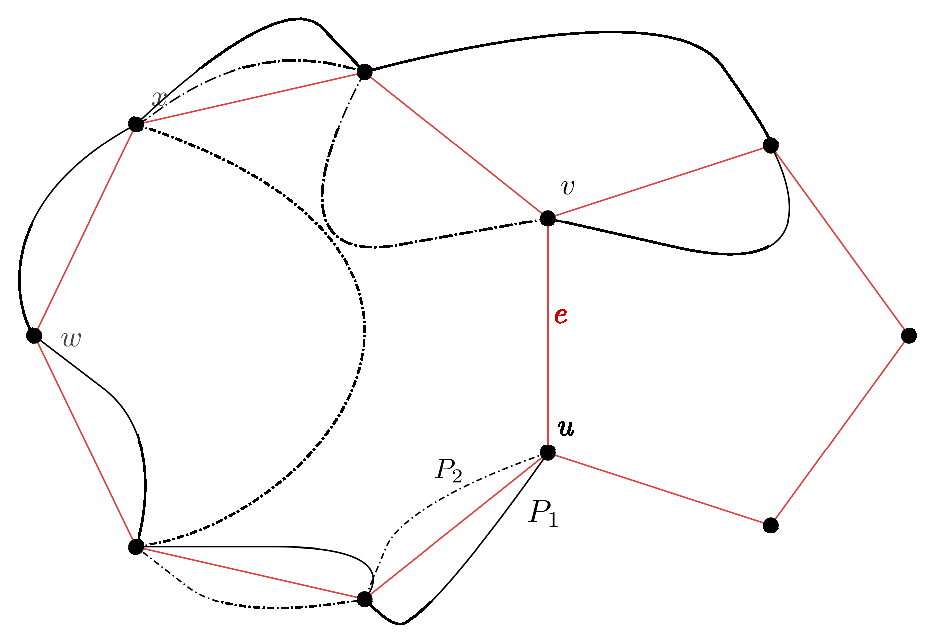
\includegraphics[scale=0.5]{Figures/Chapter1/cycle_matroid.eps}
                \caption{The cycle matroid corresponding to the graph $G$ of
                example $1.2$. Path $P_1$ is indicated by a solid line, and path
                $P_2$ indicated by a dotted line.}
                \label{fig_1.1}
            \end{figure}

        \item[(2)] Consider the graph in figure \ref{fig_1.2}, and the cycle
            matroid $M$ on $G$. The set of circuits  $\Cc$ is given by the
            collection:
            \begin{align*}
                \{e_3\} && \{e_1,e_4\} && \{e_1, e_2, e_5\} && \{e_2,e_4,e_5\} \\
            \end{align*}
            \begin{figure}[h]
                \centering
                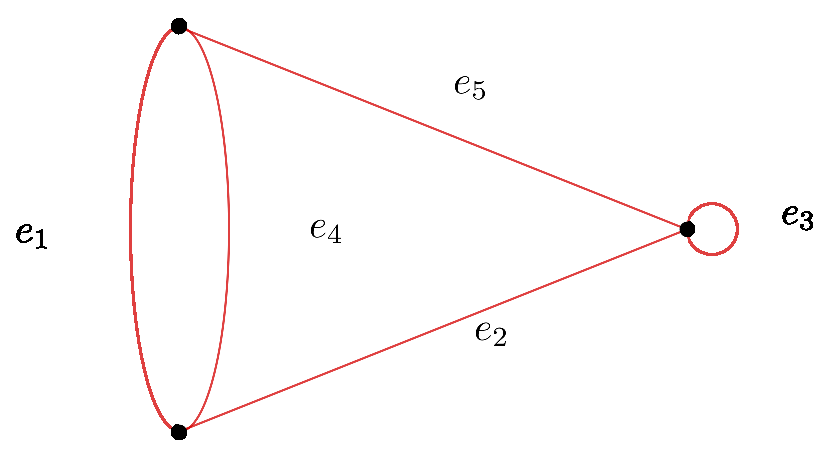
\includegraphics[scale=0.5]{Figures/Chapter1/graphic_matroid.eps}
                \caption{}
                \label{fig_1.2}
            \end{figure}
            Comparing this with the previous matroid $M'$ on the $2 \times 5$
            matrix $A$ from example $1.1(2)$. We can see that they have the same
            structure. Take the map $\psi:i \rightarrow e_i$, which is $1-1$ and
             onto, then a set  $X \subseteq E$ is a circuit in  $M$ if, and only
             if it is a circuit in $M'$.
    \end{enumerate}
\end{example}

\begin{example}\label{1.6}
    Let
    \begin{equation*}
        A=\begin{pmatrix}
            1 & 0 & 0 & 1 & 1 & 0 \\
            0 & 1 & 0 & 1 & 0 & 1 \\
            0 & 0 & 1 & 0 & 1 & 1 \\
          \end{pmatrix}
    \end{equation*}
    and let $M_2(A)$ and $M_3(A)$ be the matroids on $A$ over  $\F_2$ and
    $\F_3$, respectively. We can list the set of circuits of $M_2(A)$ to be:
    \begin{align*}
        \{1,2,4\} && \{1,3,5\} && \{2,3,6\} && \{ 4,5,6\} \\
                  && \{1,4,3,6\} && \{1,5,2,6\} && \{2,4,3,5\} \\
    \end{align*}
    while the set of circuits of $M_3(A)$ is:
    \begin{align*}
        \{1,2,4\} && \{1,3,5\} && \{2,3,6\} \\
        \{1,4,3,6\} && \{1,5,2,6\} && \{2,4,3,5\} \\
    \end{align*}
    So we can clearly see that the circuits of $M_2(A)$ and $M_3(A)$ are not the
    same. In fact, $ M_2(A)$ ia grpahic while $ M_3(A)$ is not. We also see that
    $M_2(A)$ is $\F_3$-representable, taking $A'=2A$, while $M_3(A)$ is not
    $\F_2$ -representable.
\end{example}

The above example leads us to define what we mean by a matroid isomorphism. We
present some definitions.

\begin{definition}
    We call two matroids $M_1$ and $M_2$, with ground sets $E_1$ and $E_2$,
    respectively, \textbf{isomorphic} if there exists a $1-1$ map  $\psi:E_1
    \rightarrow E_2$ of $E_1$ onto $E_2$ such that $X$ is independent in
    dependent in $E$ if, and only if  $\psi(X)$ is independent in $E_2$. We
    write $M_1 \simeq M_2$ and call $\psi$ an  \textbf{isomorphism} of the
    matroids.
\end{definition}

\begin{definition}
    Let $G$ be a graph with edge set $E$. We call the matroid on $E$ having
    $\Cc$ the collection of all egde-set defined cycles the  \textbf{cycle
    matroid} of $G$. We call a matroid  $M$  \textbf{graphic} if it is
    isomorphic to the cycle matroid of some graph.
\end{definition}

\begin{definition}
    We call a matroid \textbf{$F$-representable} if it is isomorphic to some
    vector matroid over a field  $F$. We call the ground set of the vector
    matroid a \textbf{$F$-representation}.
\end{definition}

\begin{example}\label{1.7}
    \begin{enumerate}
        \item[(1)] The matroid on the $2 \times 5$ matrix $\R$ of example
            $1.1(2)$ is $\R$-representable. It is also $\F_2$-representable.

        \item [(2)] The above matroid is a graphic matroid, isomorphic to the
            cycle matroid of example $1.2(2)$; as a consequence, that cycle
            matroid is also $\F_2$-representable.

        \item[(3)] Let $M_1$ and $M_2$ be isomorphic matroids via a map $\psi$.
            Then if  $\Ic$ is the collection of independent sets of $M_1$,
            then $\psi(\Ic)$ the collection of independent sets of $M_2$.
    \end{enumerate}
\end{example}

\begin{lemma}\label{1.1.4}
    Let $M_1$ and $M_2$ be matroids with ground sets $E_1$ and $E_2$. If $M_1
    \simeq M_2$ via the map $\psi$, then $C \subseteq E_1$ is a circuit of $M_1$
    if, and only if $\psi(C) \subseteq E_2$ is a circuit of $M_2$.
\end{lemma}
\begin{proof}
    Let $\Ic_1$ and $\Ic_2$ be the independent sets of $M_1$ and $M_2$,
    respectively, and let $C$ be a circuit of  $M_1$. Now, if $\psi(C) \in
    \Ic_2$, then by definition, we must have $C \in \Ic_1$, which contradicts
    that $C$ is a circuit. Thus  $\psi(C)$ must be a dependent set. Now, by
    definition, $C$ is minimaly dependent, so  $\com{C}{e} \in \Ic_1$, thus
    $\psi(\com{C}{e}) \in \Ic_2$. Notice, then that $\com{\psi(C)}{\psi(e)}
    \subseteq \psi(\com{C}{e})$, so by inehritance, $\com{\psi(C)}{\psi(e)} \in
    \Ic_2$. So we have that for $\psi(e) \in E_2$, $\com{\psi(C)}{\psi(e)}$ is
    independent, but $\psi(C)$ is dependent. This makes $\psi(C)$ minimally
    dependent, and thus, by definition, a circuit.
\end{proof}
\begin{corollary}
    If $\Cc_1$ and $\Cc_2$ are the collection of circuits of $M_1$ and $M_2$,
    respectively, then $\Cc_2=\psi(\Cc_1)$.
\end{corollary}
\begin{proof}
    Take the above lemma together with the fact that $\psi$ is onto.
\end{proof}

Since a matroid is determined by its ground set, there is no loss of generality
in refering to the ground set as the matroid itself, implying that we are
imposing a collection of independent sets/circuits.

\begin{definition}
    Let $M$ be a matroid. We call an element $e \in M$ a  \textbf{loop} if the
    singleton $\{e\}$ is a circuit of $M$. We call two elements  $f,g \in M$
     \textbf{parallel} if the doubleton $\{f,g\}$ is a circuit of $M$ and we
     write  $f\|g$. We define a \textbf{parallel class} of $M$ to be a maximal
     subset  $X \subseteq M$ with the property that: if  $f,g \in X$ distinct,
     then $f\|g$, and no element of  $X$ is a loop. We call a parallel class of
     $M$  \textbf{trivial} if it contains only one element. We call a matroid
     \textbf{simple} if it cntains no loops, nor parallel elements.
\end{definition}

\begin{example}\label{1.7}
    Let $A \in F^{m \times n}$ is an $m \times n$ matrix, and consider the
    vector matroid o $A$ whose independent sets are linearly independent
    columns. Since any single nonzero column of  $A$ is linearly independent, we
    have the only loop in the matroid on  $A$ is the zero-column
    $(0 \dots 0)^T$. Likewise, the parellel elements of the matroid on $A$ are
    simply the linearly dependent pairs of columns.
\end{example}

\begin{theorem}[The Strong Circuit Elimination Axiom.]\label{1.1.5}
    Let $M$ be a matroid with collection of circuits  $\Cc$. If  $C_1, C_2
    \subseteq \Cc$ are distinct, such that $e \in C_1 \cap C_2$, and $f \in
    \com{C_1}{C_2}$ then there exists a circuit $C \in \Cc$ such that  $f \in C
    \subseteq \com{(C_1 \cup C_2)}{e}$.
\end{theorem}

We now introduce one last example of a matroid for this section.

\begin{example}\label{}
    Consider the following bipartition of the sets $X=\{1,2,3\}$ and
    $Y=\{a,b,c,d,e,f\}$, together with the relation $E=\{(1,a), (2,a), (2,b),
        (2,c), (3,a), (3,b), (3,a), (3,e), (3,e)\}$. We can represent this as
        the following bipartite graph, $G=(X \cup Y, E)$ in figure \ref{fig_1.3}
    \begin{figure}[h]
        \centering
        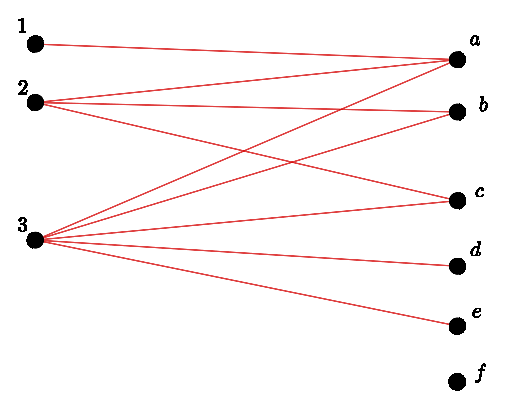
\includegraphics[scale=0.5]{Figures/Chapter1/matching.eps}
        \caption{}
        \label{fig_1.3}
    \end{figure}
    Then if we define those ``independent sets'' $\Ic$ consisting of all subsets
    of  $Y$ that can be ``matched'' to elements of $X$. i.e. those subsets of
    $Y$ whose edges between $X$ contain no incident edges. Then $Y$ together with
    $\Ic$ forms a matroid.
\end{example}

\begin{definition}
    Let $G$ be a bipartite graph with bipartition $(X,Y)$. For a subset $U$  of
    $Y$, if  $E$ is the set of edges on $ (X,U)$, then we call $E$ a
    \textbf{matching} between $X$ and  $U$ if no two edges in  $E$ have a common
    endpoint. We say that $U$ can be \textbf{matched} to $X$. We say that  $E$
    is a complete matching if $U=Y$.
\end{definition}

\begin{lemma}\label{1.1.6}
    Let $G$ be a bipartite graph, with bi-partition $(X,Y)$. Let $\Ic$ be the
    collection of all subsets of  $Y$ that can be matched to $X$. Then
    $M=(Y, \Ic)$ forms a matroid.
\end{lemma}
\begin{proof}
    We have that for $\emptyset \subseteq Y$, there are no two edges on the
    bipartition $(X,\emptyset)$ with a common endpoint; infact, there are no
    edges in this bipartition. now suppose that $I \subseteq Y$ can be matched
    to  $X$, that means no two edges between the bipartition  $(X,I)$ has a
    common endpoint. Now, if $I' \subseteq I$, then it follows that no two edges
    between  $(X,I')$ has a common endpoint. Therefore (I1), and (I2) are
    satisfied.

    Now suppose subsets $I$ and  $I'$ of $Y$ can be matched to $X$, and that
    $|I|<|I'|$. Then the bipartitions $(X,I)$ and $(X,I')$ have no two edges
    incident to each other. Then the bipartition $(X,I \cup I')$ have no two
    edges incident with each other. Now, choose an $e \in \com{I'}{I}$, then the
    edge from $e$ to some point in  $X$ has no other incident edge, therefore
    the edges between  $X$ and  $I \cup e$ have no two edges incident. That is
    no two edges are incident between $(X, I \cup e)$, therefor (I3) is
    satisfied. This makes $M=(Y,\Ic)$ into a matroid.
\end{proof}
\begin{remark}
    Notice that we can make $G$ into a bi-partite graph by taking the set of
    edges to be all matchings from the set  $X$ to subsets of  $Y$. Matroids of
    this type are called ``transversal'' and will be studied in more rigor later.
\end{remark}
